%%% LaTeX Template: Article/Thesis/etc. with colored headings and special fonts
%%%
%%% Source: http://www.howtotex.com/
%%% Feel free to distribute this template, but please keep to referral to http://www.howtotex.com/ here.
%%% February 2011t
%%%
%%% Last updated September 2021 by CDM

%%%  Preamble
\documentclass[11pt,letterpaper]{article}
%%% Our packages
\usepackage{float}

%%% Existing packages
\usepackage[margin=1.0in]{geometry}
\usepackage[T1]{fontenc}
\usepackage[bitstream-charter]{mathdesign}					
\usepackage{amsmath}						
\usepackage{xcolor}
\usepackage{cite}
\usepackage{hyphenat}
\usepackage{graphicx}
\usepackage{float}
\usepackage{subfigure}
\usepackage{sectsty}
\usepackage[compact]{titlesec} 
\usepackage[tablegrid]{vhistory}
\allsectionsfont{\color{accentcolor}\scshape\selectfont}

%%% Definitions
\definecolor{accentcolor}{rgb}{0.0,0.0,0.5} 
\newcommand{\teamname}{LJCJ}
\newcommand{\productname}{UR5/RV8}
\newcommand{\coursename}{CSE 4316: Senior Design I}
\newcommand{\semester}{Fall 2024}
\newcommand{\docname}{Project Charter}
\newcommand{\department}{Department of Computer Science \& Engineering}
\newcommand{\university}{The University of Texas at Arlington}
\newcommand{\authors}{ Luis Contreras \\ Joshua Dominguez \\ Christopher Gonzalez \\ Jasper Gustafson }

%%% Headers and footers
\usepackage{fancyhdr}
	\pagestyle{fancy}						% Enabling the custom headers/footers
\usepackage{lastpage}	
	% Header (empty)
	\lhead{}
	\chead{}
	\rhead{}
	% Footer
	\lfoot{\footnotesize \teamname \ - \semester}
	\cfoot{}
	\rfoot{\footnotesize page \thepage\ of \pageref{LastPage}}	% "Page 1 of 2"
	\renewcommand{\headrulewidth}{0.0pt}
	\renewcommand{\footrulewidth}{0.4pt}

%%% Change the abstract environment
\usepackage[runin]{abstract}			% runin option for a run-in title
%\setlength\absleftindent{30pt}			% left margin
%\setlength\absrightindent{30pt}		% right margin
\abslabeldelim{\quad}	
\setlength{\abstitleskip}{-10pt}
\renewcommand{\abstractname}{}
\renewcommand{\abstracttextfont}{\color{accentcolor} \small \slshape}	% slanted text

%%% Start of the document
\begin{document}

%%% Cover sheet
{\centering \huge \color{accentcolor} \sc \textbf{\department \\ \university} \par}
\vspace{1 in}
{\centering \huge \color{accentcolor} \sc \textbf{\docname \\ \coursename \\ \semester} \par}
\vspace{0.5 in}
\begin{figure}[h!]
	\centering
   	
\includegraphics[scale=1]{images/LJCJ.jpg}
   	
   	
   	
   	
\end{figure}
\vspace{0.35 in}
{\centering \huge \color{accentcolor} \sc \textbf{\teamname \\ \productname} \par}
\vspace{0.5 in}
{\centering \large \sc \textbf{\authors} \par}
\newpage


%\vspace{1 in}
%\centerline{January 13th, 2012}
%\newpage

%%% Revision History
\begin{versionhistory}
  	\vhEntry{0.1}{09.22.2024}{JG}{document creation}
  	\vhEntry{0.2}{09.26.2024}{LC}{sections 1-3}
  	\vhEntry{0.3}{09.28.2024}{JG}{milestones}
  	\vhEntry{0.4}{09.29.2024}{JG|CG|JD}{sections 5-8, 11-13, 14}


\end{versionhistory}
\newpage

%%% Table of contents
\tableofcontents


\newpage

%%% List of figures and tables (optional)
\listoffigures

%\listoftables
\newpage
\section{Problem Statement}
The transition to smart manufacturing presents significant challenges that hinder the full realization of its potential benefits. Smart manufacturing relies on the integration of advanced technologies, such as IoT, artificial intelligence and data analytics, to optimize production processes, enhance flexibility, and improve overall efficiency. However, many manufacturers struggle with issues such as legacy systems, data silos, insufficient workforce training, and cybersecurity vulnerabilities. These challenges result in suboptimal production performance, increased downtime, and higher operational costs, ultimately impacting competitiveness in a rapidly evolving market. There is a pressing need to identify and address the barriers to implementing smart manufacturing solutions effectively.
\section {Methodology}
The objective of this project is to enhance the capabilities of an RV8 robot work cell by integrating various component
, including an end-effector (gripper), a laser safety scanner, emergency stop (E-stop) switches, a MELSEC PLC controller
, a host PC, and a linear rail. The integration aims to facilitate advanced control applications such as pick and place,
palletizing, and depalletizing while ensuring compliance with safety standards.
Currently, the work cell lacks the necessary components and configurations to operate efficiently and safely in a
dynamic environment. The project will focus on developing a robust control application that not only enables the desired
robotic operations but also incorporates critical safety features, including safety cutoffs and direct entry presence
detection. This integration is vital to minimize operational risks and enhance productivity within the work cell.By
addressing these goals, the project aims to transform the RV8 robot work cell into a highly capable, safe, and efficient
automated solution for industrial applications
\section{Value Proposition}
To address the challenges of smart manufacturing, a structured methodology will be implemented, starting with a comprehensive assessment of current manufacturing processes, technologies, and workforce capabilities. This phase will involve gap analysis and technology audits to identify integration needs. Following this, a detailed technology road-map will be developed to facilitate the seamless integration of advanced technologies with legacy systems, supported by pilot projects for real-world validation.

Simultaneously, a targeted workforce development program will be designed to close skill gaps, focusing on training in new technologies and cybersecurity best practices. A robust cybersecurity framework will be established through risk assessments and regular audits. Finally, key performance indicators (KPIs) will be defined to measure success, alongside a feedback mechanism for continuous improvement. This systematic approach aims to enable organizations to transition effectively to smart manufacturing, enhancing efficiency and competitiveness in the market.
\newpage
\section{Development Milestones}
The following is a list of completion dates for all major documents, demonstrations, and associated deadlines:
\begin{itemize}
  \item Project Charter Final Draft             - September 30, 2024
  \item System Requirements Specification       - October   21, 2024
  \item Architectural Design Specification      - November   4, 2024
  \item Demonstration of MELSEC PLC Programming - November,     2024
  \item Demonstration of E-Stop Switch          - November,     2024
  \item Demonstration of Laser Safety Scanner   - December,     2024
  \item Demonstration of Linear Rail Movement   - January,      2025
  \item Demonstration of Gripper Configuration  - February,     2025
  \item Demonstration of Basic Stacking         - March,        2025
  \item Demonstration of Palletizing Algorithm  - March,        2025
  \item CoE Innovation Day poster presentation  - April     16, 2025
  \item Final Project Demonstration             - April,        2025    
  \item Final Project Submission                - May        1, 2025
\end{itemize}


\setcounter{table}{0}
\newpage

%%% Remaining project charter sections
\section{Background}
%% It is just an empty TeX file.
%% Write your code here.
Historically, interactions between humans and industrial robots have been major safety concerns. Early factory environments did not focus on human safety in these conditions. This often resulted in strict separation between workers and machines, with physical barriers and lock-out protocols put in place to prevent accident or injury. These set-ups created restricted zones around machinery, and created hazardous conditions whenever human interaction or intervention with the equipment was necessary. Human intervention with a palletizing robot is often necessary for troubleshooting errors in the production line, such as a misplaced or trapped box on the conveyor belt. In these situations, workers must enter the robot’s operating zone to correct the issue, which is dangerous in traditional set-ups.

In a factory palletization setting, the UR20 Cobot offers a safety advantage compared to traditional heavy machinery. Whereas conventional automated systems which often require physical barriers or guarded zones to protect workers from potential harm, the UR20 is specifically engineered for safe human interaction. Its integrated sensors detect physical touch and respond to any notable resistance by stopping movement immediately. This built-in responsiveness drastically reduces the risk of accidents, even when the cobot is performing tasks that involve lifting heavy payloads. This makes it no longer necessary to guard the operating area with restricted zones or physical barriers, allowing for more efficient operation and greater worker safety.

Our implementation of the UR20 Cobot includes proximity detection and camera systems capable of recognizing human presence. These technologies allow the cobot to anticipate and respond to the presence of nearby workers, reducing the possibility of workplace accidents.


\section{Related Work}

Automation is an emerging state-of-the-art technology in manufacturing and logistics, advancing signinficantly year after year. These solutions are available in various forms, including academic research, commercial use, and prototypes. There are several commercial solutions to optimizing work efficiency with automated robots, each with their own strengths and weaknesses. One of the large commercially available solutions is Robotiq's robotic palletizing solution, that can be installed in days and resolve production instability \cite{Robotiq2024}. Despite the advantages, solutions such as these are very costly where the palletizing application of the RV8 would cut costs.

Robotic palletizing is also a popular topic in academic research, focusing on the algorithms for object recognition, position control, and planning \cite{Xu2022}. Additionally power consumption plays a large role in the cost of operation, and is a field that is researched to reduce operating power consumption \cite{Deng2022}. Furthermore, while many solutions claim to be easily deployable they often require substantial training on how to operate the system. The RV8 palletizing application will tackle this problem with the process and setup being documented. Industrial solutions also exist to face growing demands to improve efficiency, utilizing industrial wireless sensor networks for rapid deployment and flexibility \cite{Gungor2009}. Lastly, a major factor in the efficiency of the palletization application is the vision of the robot. The time for recognition of an object and its dimenisons are incredibly important for selection and placement \cite{Abdullah2022}. Our RV8 robot will feature a gripper and vision system to efficiently detect objects and determine the best fit location for it.

\section{System Overview}
This section should reintroduce the full data flow diagram from the architectural specification, and discuss at a high level the purpose of each layer. You do not need to include a subsection for each layer, a 1 - 2 paragraph recap is sufficient.

\begin{figure}[h!]
	\centering
 	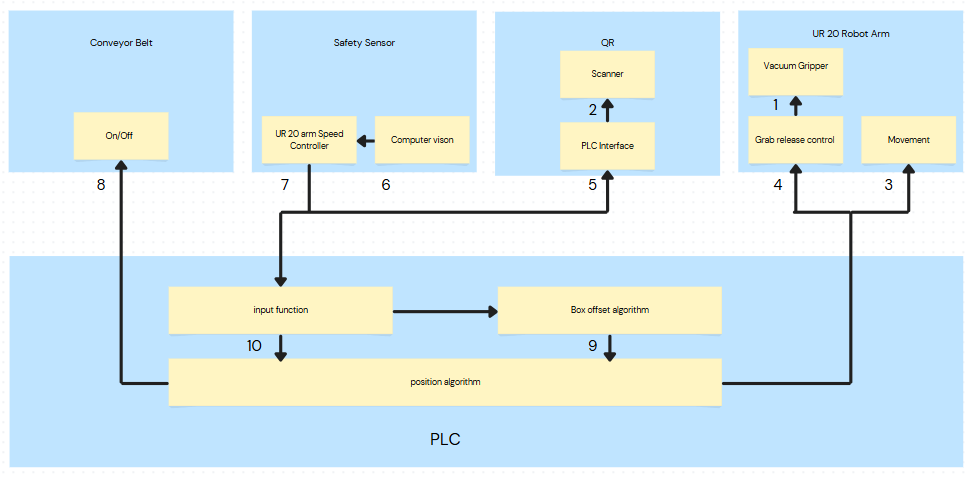
\includegraphics[width=0.90\textwidth]{images/data_flow}
 \caption{System architecture}
\end{figure}
\newpage
\section{Roles \& Responsibilities}
The stakeholders in this project are Dr. McMurrough as the sponsor and the undergraduates working on its completion. The undergraduates are two Computer Engineering majors, Luis Contreras and Jasper Gustafson, as well as two Computer Science majors, Christopher Gonzales and Joshua Dominguez.The main point of contact with Dr. McMurrough will be through Luis Contreras.Luis Contreras and Jasper Gustafson will be responsible for the hardware. This will include determining appropriate parts and necessary accessories, connecting those parts to the existing robot, and programming interfaces to enable control of the robot through the wired connections. Christopher Gonzalez and Joshua Dominguez will be responsible for the software. This will include programming behavior of the robot, including the linear rail, in combination with the palletizing algorithm.

The scrum master and speaker during presentations will rotate weekly, with one person having full control during their week. The rotation of these presentations is planned to be in the following order: Luis Contreras, Jasper Gustafson, Christopher Gonzalez, Joshua Dominguez. This order may change if someone wishes to switch their week.
\section{Cost Proposal}
This proposal will be focusing on the UR20 Cobot, although the original design was for the Mitsubishi RV8 arm.

\subsection{Current \& Pending Support}
This project's funding currently consists of only the default \$800 funding from the CSE department. More funding may be provided with sufficient justification, but no other funding sources are currently known.

    Current total funds:
    \begin{itemize}
        \item \$800 Default Budget
    \end{itemize}

\subsection{Final Budget}
The final cost of our project as of April 2025 is listed here.
The UR20 Cobot has a provided safety scanner, wiring box, and conveyor belt. A gripper will need to be purchased or designed in order for it to perform a palletizing application.

The item that ended up being chosen was a custom-design suction-cup gripper using parts borrowed from the Senior Design labs and 3D printed materials. \$300 worth of suction cups were purchased before an unused, higher-quality alternative was found in the labs.  


This table records the cost of all acquired items for the project.
\begin{table}[H]
\centering
    \caption{Budget itemization}
    \begin{tabular}{|l|l|}
        \hline
        \textbf{Item} & \textbf{Price} \\ \hline
        End effector and components & \$300+ \\ \hline
        Vacuum pump  and components & \$0 \\ \hline
        Mounting bracket & \$0\\ \hline
        Feeder belt & \$0 \\ \hline
        Photoeye detector & \$30 \\ \hline
        Miscellaneous small parts (screws, shaft collars, etc) & \$100 \\ \hline
        Raspberry Pi and camera & \$0 \\ \hline
        Boxes and pallet & \$0 \\ \hline
    \end{tabular}
\end{table}

\subsection{Preliminary Budget}
 The original options considered at the creation of this document are listed here.

\begin{itemize}
    \item A conveyor belt will likely be necessary for simulation of a real-world factory palletizing environment's margin of error.
    \item A vacuum generator will be needed, either included in the gripper or acquired separately.
    \item For palletizing, it is likely that a suction grip will be the most effective. However, those grips can be extremely expensive, likely coming in at a minimum of \$2000 unless used parts can be found. This is due to the necessity of a vacuum generator attached before the actual gripper in order to provide it power.
    \item Some more light-weight grippers have been designed for other robots such as MyCobot, and may be translatable to our robot. This would cost only \$400, and should be explored by reaching out to those manufacturers for questions.
    \item We could also, as the most time-consuming option, take inspiration from existing designs of vacuum pumps or end effectors and design one of the components, using the remaining money to invest in the other component. 
\end{itemize}


This table assumes we will purchase the cheapest versions of the above options instead of making them ourselves.
\begin{table}[H]
\centering
    \caption{Budget planning}
    \begin{tabular}{|l|l|}
        \hline
        \textbf{Item} & \textbf{Price} \\ \hline
        End effector and components & \$400+ \\ \hline
        Vacuum pump  and components & \$200+ \\ \hline
        Mounting bracket & \$100\\ \hline
        Feeder belt & \$100 \\ \hline
    \end{tabular}
\end{table}

\section{Facilities \& Equipment}
%% It is just an empty TeX file.
%% Write your code here.
The UR20 Palletizing Cobot project is located in ERB 335, a designated laboratory area. A rectangular area approximately 10x5 feet in dimension is necessary for palletizing. For safety reasons, the robot will not operate if any obstacle, especially a person, is within this radius. The lab area includes the appropriate electrical infrastructure accommodating the power requirements of the UR20 robot. It will be necessary for the robot to be bolted into the ground for safe operation. This will be handled by the lab coordinator.

Equipment needed includes 3D printers (already present in the lab), a conveyor belt (already present in the lab), an air compressor (already present in the lab). Materials needed to conduct testing will be a pallet (borrowed from UTA) and boxes of consistent dimensions (printer paper boxes borrowed from UTA). 

Components will be 3D printed or purchased using the team budget. Circuits will be made by team members using materials borrowed from UTA Senior Design labs. If time and budget permits, some components will be finalized as aluminum parts, as opposed to 3D printed material. Some equipment will be provided by team members, such as a Raspberry Pi used for the human shape recognition camera stretch goal.
\section{Assumptions}
\begin{itemize}
  \item The robot used for our project will be the Mitsubishi RV-8CRL-D arm
  \item The safety scanner will be provided, along with the robot arm
  \item The gripper suitable for palletizing will be purchased/designed by the 3rd sprint cycle 
  \item There will be sufficient space in ERB 335 for the robot's palletizing application
  \item The Engineering Research Building will provide stable internet connectivity and sufficient power 
  \item The existing safety scanner and PLC setup is fully functional without significant reconfiguration following the integration of a gripper
  \item All necessary tools and equipment will be provided and readily available in ERB 335
\end{itemize}
\section{Constraints}
\begin{itemize}
    \item final prototype demonstration must be completed by May 1st 2025
    \item Robot arm shall only be programmed via host PC or Teaching Pendant in ERB 335
    \item UR20 testing must be done in the space of ERB 335
    \item Total development cost must not exceed \$800
\end{itemize}
% possible fix for formatting of risk table showing up in documentation section
% \newpage
\section{Risks}
\begin{table}[H]
    \resizebox{\textwidth}{!}{
    \begin{tabular}{|l|l|l|l|}
    \hline
    \textbf{Risk description} & \textbf{Probability} & \textbf{Loss (days)} & \textbf{Exposure (days)} \\ \hline
    Shipping delay on gripper parts                    & 0.50 & 30 & 15    \\ \hline
    Unable to find compatible gripper for product task & 0.05 & 40 & 2     \\ \hline
    Issues with hardware or gripper behavior           & 0.20 & 7  & 1.4    \\ \hline
    Difficulty with PLC setup or connecting to host PC & 0.20 & 5  & 1     \\ \hline
    Delay due to member being ill                      & 0.05 & 5  & .25   \\ \hline
    \end{tabular}}
    \caption{Overview of highest exposure project risks} 
\end{table}
\section{Documentation \& Reporting}

\subsection{Major Documentation Deliverables}

\subsubsection{Project Charter}
The Project Charter will be maintained in a shared GitHub repository and updated after any major changes in project scope or deadlines. The initial version will be delivered on September 30th, 2024.

\subsubsection{System Requirements Specification}
The System Requirements Specification will be maintained in a shared GitHub repository and updated as needed with any changes to the system capabilities. The document will be delivered on October 21st, 2024.

\subsubsection{Architectural Design Specification}
Architectural Design Specification will be maintained in a shared GitHub repository and updated following any changes to the system's structure. The document will be delivered on November 4th, 2024. 


\subsubsection{Detailed Design Specification}
The Detailed Design Specification will be maintained in a shared GitHub repository and updated if any significant design changes occur. The DDS document will be delivered at the end of Sprint 5 (February, 2025).

\subsection{Recurring Sprint Items}
The most common recurring sprint items will be acquisition of materials and placement/recognition algorithm testing. All other sprint items will be completable items related to design and setup.

\subsubsection{Product Backlog}
Items will be added to the product backlog based system requirements outlined in the SRS. The items will be prioritized during sprint planning meetings based on complexity and impact on ability to move forward with the project.

\subsubsection{Sprint Planning}
Each sprint will be planned during a sprint planning meeting held at the beginning of the sprint cycle. There will be 8 sprints over the course of both semesters.
\subsubsection{Sprint Goal} 
The sprint goal will be decided collaboratively during the sprint planning meeting by the development team.
\subsubsection{Sprint Backlog}
The sprint backlog will be selected from the product backlog during sprint planning, focusing on the highest-priority items. The team will use spreadsheets to maintain and track the sprint backlog and update as needed.

\subsubsection{Task Breakdown}
Individual tasks will be partitioned into hardware, software, or group tasks, and an applicable team member will voluntarily claim uncompleted tasks. Time spent on tasks will be documented in a spreadsheet.

\subsubsection{Sprint Burn Down Charts}
The presentations will go in a rotation of four weeks, in the order of Luis, Jasper, Chris, Joshua. The person responsible for the presentation will also be responsible for the sprint burn-down chart. Individual members will be responsible for reporting their time, either directly to the spreadsheet or to the group. The following figure is an example of the burn down chart.

\begin{figure}[h!]
    \centering
    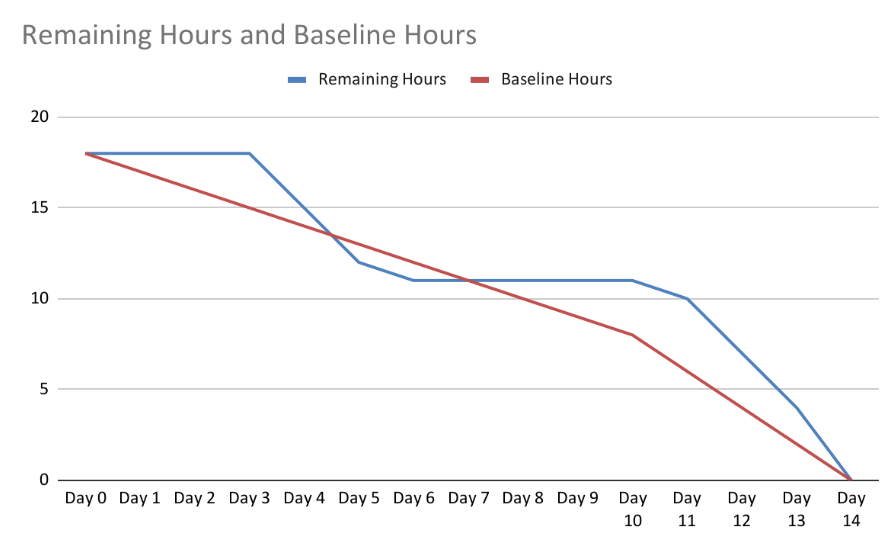
\includegraphics[width=0.5\textwidth]{images/burndown}
    \caption{Example sprint burn down chart}
\end{figure}

\subsubsection{Sprint Retrospective}
The sprint retrospective will be conducted as a team discussion at the end of each sprint. This meeting will reflect on success and areas for improvement, with all team members offering feedback. The key items will be the ways to improve, what did not work, and what did work well. The teammate responsible for that week's presentation will also be responsible for documenting the team's retrospective discussion.

\subsubsection{Individual Status Reports}
Over the sprint and during the group team retrospective, each teammate will document the hours they have worked on each task and discuss the task's completion. The relevant information will be documented individually by each teammate for their individual status report submission, including the teammate additionally responsible for the retrospective presentation.

\subsection{Closeout Materials}
The required materials will be submitted by the team in April 2025: 
\begin{itemize}
    \item Project poster
    \item CSE blog webpage
    \item Documents from 4316 and 4317
    \item Demo Videos, final demo \& extra footage
    \item Source code and documentation
    \item STL design files
    \item Circuit design files
\end{itemize}

\subsubsection{System Prototype}
The final system prototype will include the complete integration for the UR20 robot with a gripper and palletizing application. The prototype will be demonstrated by the UR20 robot palletizing boxes in ERB 335 in April 2025.
\subsubsection{Project Poster}
The project poster will include the project description, system architecture, results, and impact. It will follow standard poster dimensions (36"x48") and will be delivered in April 2025.

\subsubsection{Web Page}
The project webpage will include the project description, system requirements, demonstration videos, and deliverables. It will be provided at closeout in April 2025.

\subsubsection{Demo Video}
The video will show the UR20 robot in action performing palletizing tasks. B-reel footage will also be included for future video cuts. The video will be approximately 3-8 minutes long covering system setup, algorithms, and functionality.

\subsubsection{Source Code}
Source Code is written exclusively on the UR Teaching Pendant. Individual programs are saved and stored on the pendant, which is to be left with the UR20 to be accessible at all times. 

\subsubsection{Source Code Documentation}
Documentation will be written manually due to the nature of the UR20 Teaching Pendant.

\subsubsection{Hardware Schematics}
The hardware schematics will include wiring diagrams and any PCB layouts required for the integration of the gripper and accessory hardware.

\subsubsection{CAD files}
The project involves designing and printing a gripper, support components for the conveyor belt, and casing for the photoeye and camera. Tinkercad will be used for design. Final files will be provided in STL formats.

\subsubsection{Installation Scripts}
The programs will be handled by the teaching pendant and can be run from that source with little complication. The installation of the robot will largely involve physical installation in a location.

\subsubsection{User Manual}
A detailed user manual will be provided, including the setup steps in digital PDF format alongside a setup video demonstrating how the robot works. 
\newpage


%%% References
\bibliographystyle{plain}
\bibliographystyle{reference/IEEEtran_custom}
\bibliography{reference/refs}{}

\end{document}